% ── SLIDE 17: DEMO FALLO FRAMES ───────────────────────────────────────────────
\begin{frame}{Qualitative Demo --- Failure Case (ID Switch)}
  \begin{columns}[T]
    \begin{column}{0.32\textwidth}
      \centering
      {\small\textbf{Before occlusion}}\\[3pt]
      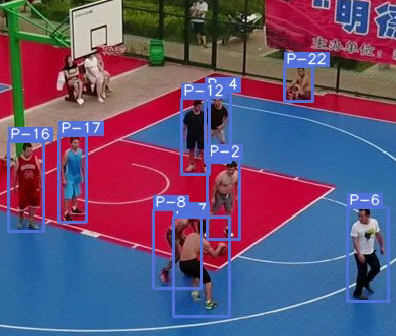
\includegraphics[width=\linewidth]{figures/yolo11_fail_f1.png}
    \end{column}
    \begin{column}{0.32\textwidth}
      \centering
      {\small\textbf{During occlusion}}\\[3pt]
      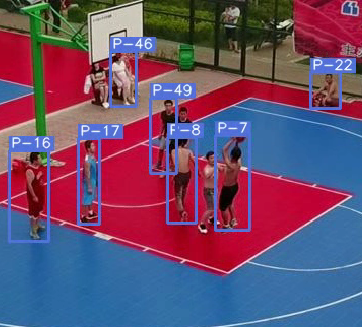
\includegraphics[width=\linewidth]{figures/yolo11_fail_f2.png}
    \end{column}
    \begin{column}{0.32\textwidth}
      \centering
      {\small\textbf{After occlusion}}\\[3pt]
      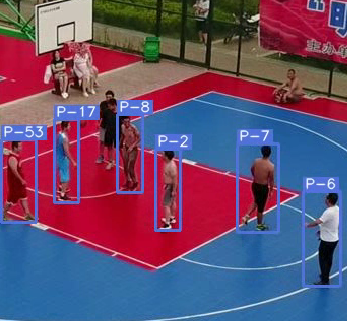
\includegraphics[width=\linewidth]{figures/yolo11_fail_f3.png}
    \end{column}
  \end{columns}
  \vspace{0.4em}
  \begin{block}{ID Switch}
    \small When an object is occluded for $>\!$ \texttt{max\_age} frames,
    SORT deletes the track. On reappearance, no Kalman prediction
    is available $\Rightarrow$ a new ID is assigned.
  \end{block}
\end{frame}

